% =========================================================================
% SECTION 2: PRISM SYSTEM ARCHITECTURE
% =========================================================================
\section{PRISM System Architecture}
\label{sec:architecture}

PRISM processes camera and inertial sensor inputs through an autonomous, unidirectional pipeline running natively on Android (Fig.~\ref{fig:pipeline_architecture}). The architecture decouples image acquisition, geometric reconstruction, kinematic tracking, collision arbitration, and multimodal guidance into modular stages.

% Figure 1: PRISM Android System Pipeline Architecture (Monochrome 300 DPI)
\begin{figure}[!t]
\centering
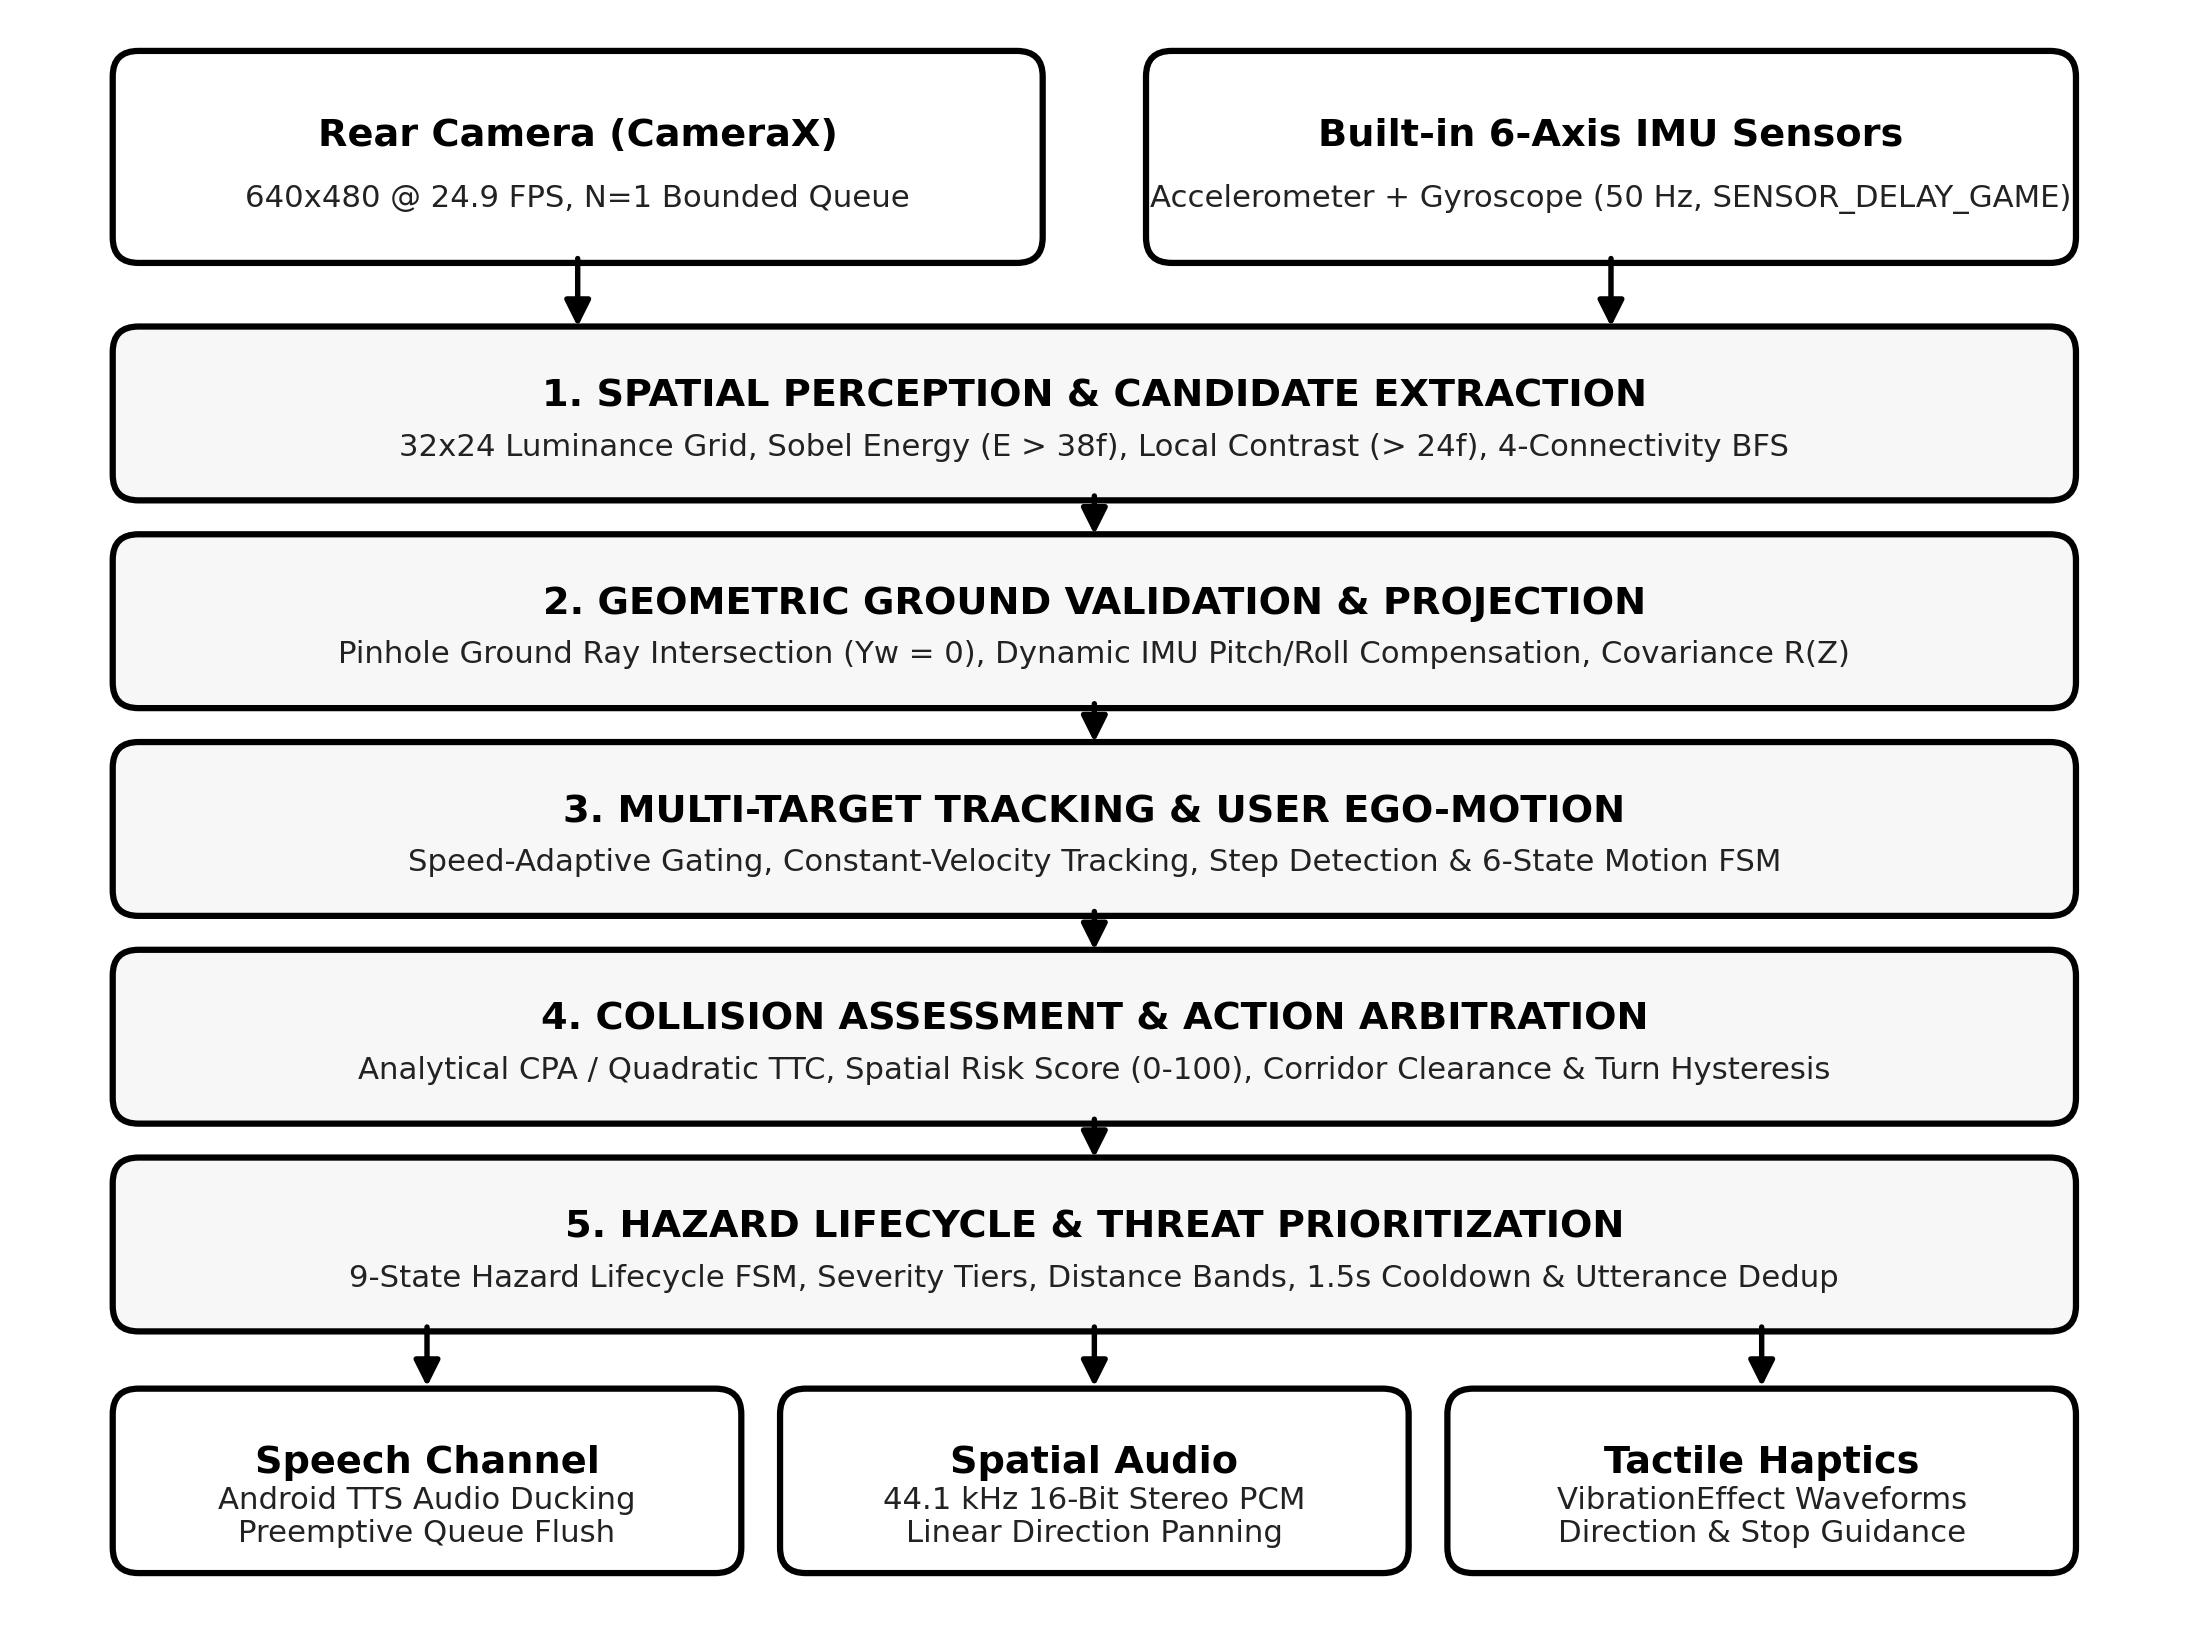
\includegraphics[width=\columnwidth]{figures/fig_pipeline.png}
\caption{PRISM Android system pipeline architecture (black and white): unidirectional execution flow from CameraX image acquisition and IMU sensor registration through spatial candidate extraction, geometric ground projection, multi-target tracking, hazard lifecycle arbitration, multimodal presentation, and telemetry streaming.}
\label{fig:pipeline_architecture}
\end{figure}


The software architecture follows four design principles:
\begin{enumerate}
    \item \textbf{Forward-Only Dataflow}: Information travels strictly downstream from sensor drivers to output actuators without circular dependencies or backward state mutation.
    \item \textbf{Immutable Typed Contracts}: Subsystems exchange immutable Kotlin data classes (\texttt{CandidateCluster}, \texttt{TrackInfo}, \texttt{PrismDecision}, \texttt{SpatialCue}), ensuring thread-safe transfers across coroutine scopes.
    \item \textbf{Ground-Plane Metric Space}: Spatial tracking, kinematics, and corridor bounds operate in Cartesian coordinates $(X, Z) \in \mathbb{R}^2$ referenced to the floor nadir directly below the camera.
    \item \textbf{Bounded Backpressure}: The vision loop enforces a single-frame buffer ($N = 1$) via CameraX \texttt{STRATEGY\_KEEP\_ONLY\_LATEST}, dropping stale frames to prevent latency accumulation.
\end{enumerate}

% Table 1: Frozen PRISM Android System Configuration Parameters (PRISM-L1.0)
\begin{table}[!t]
\caption{Frozen PRISM-L1.0 Android System Configuration Parameters}
\label{tab:configuration}
\centering
\scriptsize
\setlength{\tabcolsep}{2pt}
\begin{tabularx}{\columnwidth}{p{1.9cm}p{1.7cm}X}
\toprule
\textbf{Subsystem} & \textbf{Parameter} & \textbf{Value / Operational Rule} \\
\midrule
\textbf{CameraX \& Frame}
  & Backpressure policy & \texttt{KEEP\_ONLY\_LATEST} ($N=1$ frame) \\
  & Stale frame limit   & $\Delta t > 0.25$\,s $\to$ \texttt{DEGRADED} state \\
  & Luminance grid      & $32 \times 24$ subsampling grid on Y-plane \\
\midrule
\textbf{Perception \& Geometry}
  & Energy / Contrast   & Sobel $E > 38f$, local contrast $> 24f$ \\
  & Cluster / Mounting  & $\ge 6$ cells; $h = 1.30$\,m, $\theta_p = 12^\circ$ \\
  & Metric bounds       & $Z \in [0.4, 6.5]$\,m; Corridor $|X| \le 1.25$\,m \\
  & Physical dimensions & $H \in [0.32, 2.4]$\,m, $W \in [0.1, 2.2]$\,m \\
  & Covariance model    & $R(Z) = 0.04 + 0.015 Z$ \\
\midrule
\textbf{Tracking \& Fusion}
  & Association gating  & $d_{\text{gate}} = \max(0.9, \min(1.8, 1.0 + 2.0 v \Delta t))$\,m \\
  & Track lifecycle     & $\ge 2$ hits confirm ($Z < 1$\,m instant), coast 5 frames \\
  & Velocity clamp      & $|V_x| \le 3.5$, $|V_z| \le 4.5$\,m/s (EMA $\alpha = 0.50$) \\
  & Orientation fusion  & Gyro integration + gravity drift ($\alpha = 0.05$) \\
  & Step detection      & Peak $1.20$\,m/s$^2$, refractory period $0.28$\,s \\
  & Motion energy RMS   & Stationary $< 0.25$\,m/s$^2$; Active $> 0.60$\,m/s$^2$ \\
\midrule
\textbf{Hazard \& Warning}
  & Action boundaries   & Emergency $Z < 1.0$\,m / $S \ge 85$; Evasion $Z < 2.6$\,m \\
  & Turn hysteresis     & $\Delta C = 0.15$ cost barrier; heading $\pm 0.45$\,rad \\
  & Multimodal output   & 44.1\,kHz stereo PCM, TTS ducking, 1.5\,s cooldown \\
\bottomrule
\end{tabularx}
\par\smallskip{\raggedright \tiny Frozen snapshot from \texttt{PRISM-L1.0-config.json} and Kotlin implementation.\par}
\end{table}


\subsection{Android Host and Runtime Lifecycle}
The application structure pairs \texttt{PrismApplication} for dependency lifecycle management with \texttt{MainActivity} for user interaction. The interface provides a Jetpack Compose dashboard (\texttt{PrismScreen}, Fig.~\ref{fig:app_interface}) featuring high-contrast banners, live camera corridor view, and accessible controls. \texttt{PrismRuntime} coordinates concurrent coroutines that ingest CameraX frames, listen for IMU events via \texttt{SensorEventListener}, dispatch multimodal guidance, and stream JSONL telemetry on port 8080.

% Figure 2: PRISM Android Live Application Interface (Physical Device Screenshot)
\begin{figure}[!t]
\centering
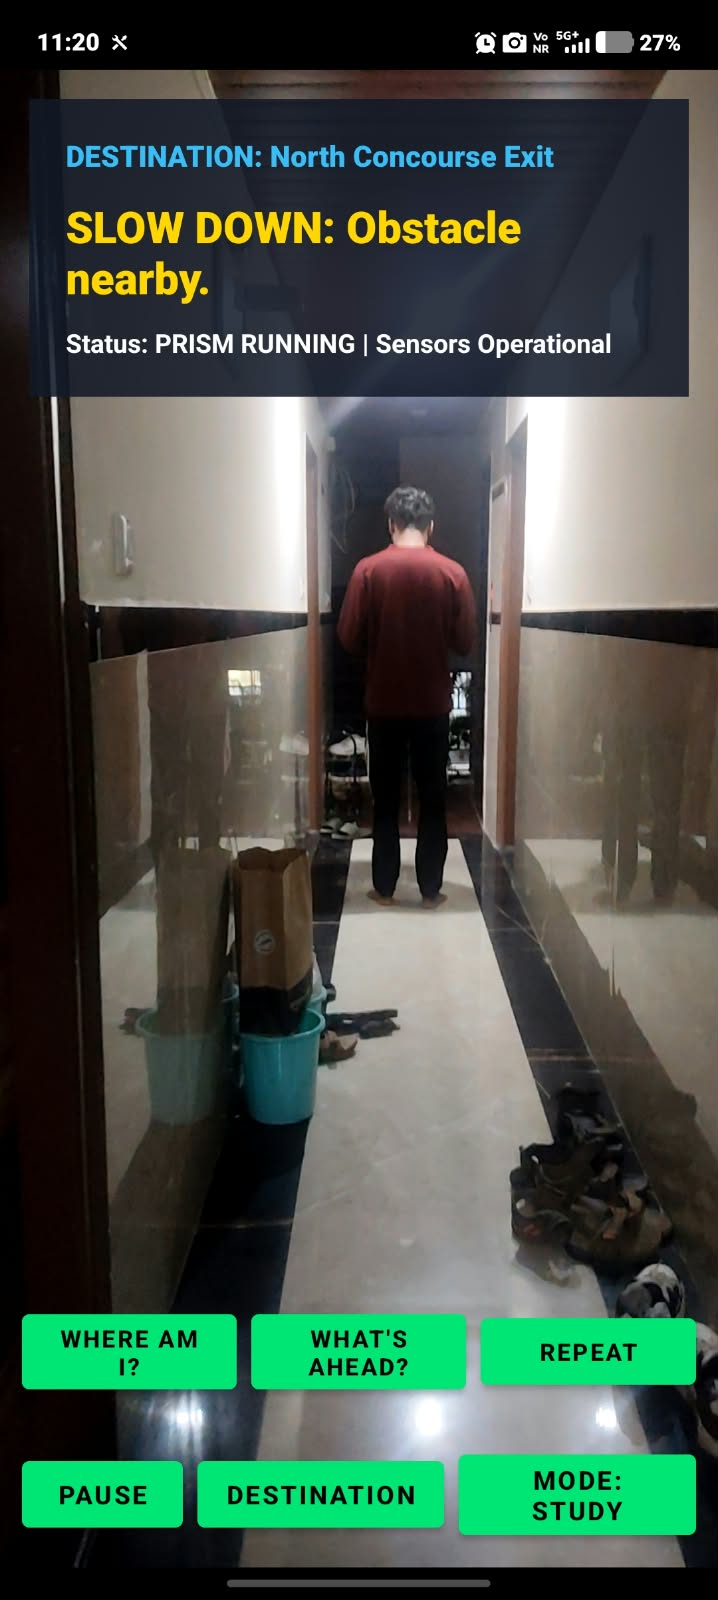
\includegraphics[width=0.60\columnwidth]{figures/app_interface.jpg}
\caption{PRISM Android live application interface on physical device: top high-contrast guidance banner (\texttt{SLOW DOWN: Obstacle nearby.}), real-time camera view tracking an in-path pedestrian obstacle during indoor corridor navigation, and accessible touch controls (\texttt{MODE: STUDY}).}
\label{fig:app_interface}
\end{figure}


The runtime manages three operational states: \texttt{RUNNING} (nominal processing), \texttt{DEGRADED} (sensor dropout or frame interval $\Delta t > 0.25$\,s, falling back to proximity thresholding), and \texttt{STOPPED} (unbound listeners). Clock skew causing negative intervals ($\Delta t < 0$) commands an immediate fail-safe \texttt{EMERGENCY\_STOP}. System constants are frozen in \texttt{PRISM-L1.0-config.json}~\cite{PRISM-L1.0-config,PRISM-L1.0-README} (Table~\ref{tab:configuration}).
